\documentclass[aspectratio=169,10pt]{beamer}

\usepackage[utf8]{inputenc}
\usepackage{graphicx}
\usepackage{booktabs}
\usepackage{array}
\usepackage{xcolor}
\usepackage{ragged2e}
\usepackage{tikz}
\usepackage{tabularx}

\usetheme{Madrid}
\usecolortheme{default}
\setbeamertemplate{navigation symbols}{}
\setbeamertemplate{caption}[numbered]

\definecolor{bg}{HTML}{FFFFFF}
\definecolor{bg2}{HTML}{F4F7FB}
\definecolor{fg}{HTML}{1F2937}
\definecolor{navy}{HTML}{0F172A}
\definecolor{muted}{HTML}{6B7280}
\definecolor{accent}{HTML}{2563EB}
\definecolor{accent2}{HTML}{B45309}

\setbeamercolor{normal text}{fg=fg,bg=bg}
\setbeamercolor{structure}{fg=accent}
\setbeamercolor{frametitle}{fg=navy,bg=bg}
\setbeamercolor{title}{fg=navy,bg=bg}
\setbeamercolor{alerted text}{fg=accent2}
\setbeamercolor{block title}{fg=navy,bg=bg2}
\setbeamercolor{block body}{fg=fg,bg=bg2}
\setbeamertemplate{background canvas}{\color{bg}}

\setlength{\parskip}{0.25em}

\newcommand{\pill}[1]{\tikz[baseline=(X.base)]\node[draw=gray!25,rounded corners=2.4pt,fill=gray!10,inner xsep=7pt,inner ysep=2.2pt](X){\strut\footnotesize #1};}
\newcommand{\bigmetric}[3]{\begin{beamercolorbox}[wd=\linewidth,rounded=true,sep=0.95em,center]{block body}\textcolor{muted}{\small #1}\par\vspace{0.28em}{\Large\bfseries #2}\par\vspace{0.18em}{\scriptsize #3}\end{beamercolorbox}}
\newcommand{\smallcard}[2]{\begin{beamercolorbox}[wd=\linewidth,rounded=true,sep=0.6em]{block body}\textcolor{muted}{\scriptsize #1}\par{\small\bfseries #2}\end{beamercolorbox}}
\newcommand{\metricstrip}[3]{\begin{beamercolorbox}[wd=0.235\linewidth,rounded=true,sep=0.45em,center]{block body}\textcolor{muted}{\scriptsize #1}\par{\normalsize\bfseries #2}\par{\scriptsize #3}\end{beamercolorbox}}
\newcommand{\sectionlabel}[1]{\textcolor{accent}{\small\bfseries\uppercase{#1}}}

\title{Gemini Is All You Need}
\author{SEG 4180 Project Report}
\date{}

\begin{document}

\begin{frame}[plain]
	\vspace*{0.2em}
	\begin{columns}[T,onlytextwidth]
		\column{0.45\textwidth}
		\vspace{0.35em}
		{\Huge\bfseries Gemini Is All You Need\par}
		{\Large\bfseries Synthetic-only vehicle detection\par}

		\vspace{0.6em}
		\small{A leakage-safe synthetic pipeline produced a strong detector on held-out Street View.}

		\column{0.55\textwidth}
		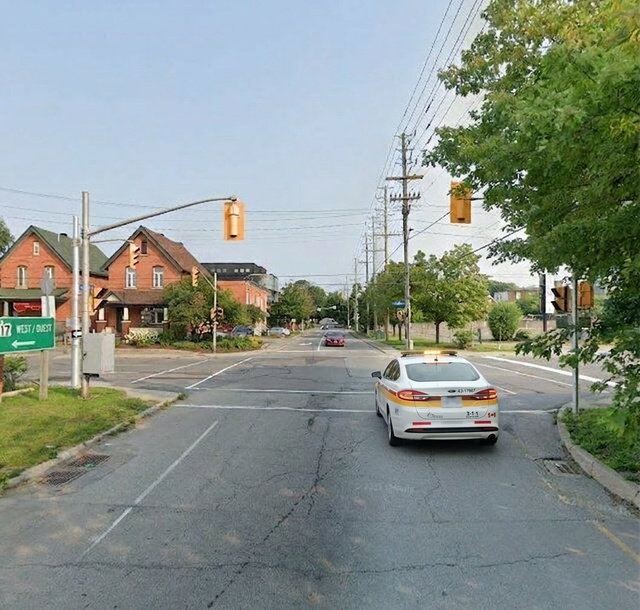
\includegraphics[width=\linewidth,height=0.74\textheight,keepaspectratio]{synthetic-enforcement.jpg}
	\end{columns}
\end{frame}

\begin{frame}{Why this mattered}
	\begin{block}{Problem}
		\begin{itemize}
			\item Enforcement vehicles are rare.
			\item Manual collection is slow and expensive.
			\item Synthetic data provided control.
		\end{itemize}
	\end{block}

	\vspace{0.35em}
	\begin{center}
		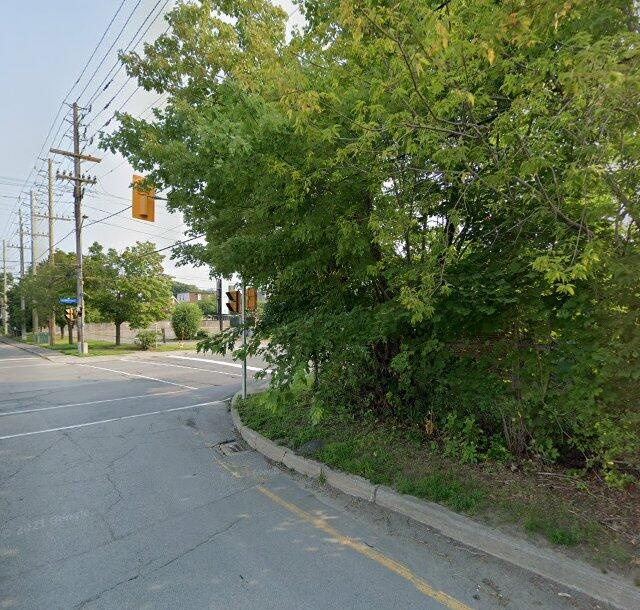
\includegraphics[width=0.80\linewidth,height=0.42\textheight,keepaspectratio]{street-view-empty.jpg}
		\par\vspace{0.15em}
		{\scriptsize\textcolor{muted}{A real Street View scene from the report's baseline imagery.}}
	\end{center}
\end{frame}

\begin{frame}{Pipeline}
	\begin{center}
		\begin{minipage}{0.95\linewidth}
			\begin{columns}[T,onlytextwidth]
				\column{0.49\textwidth}\smallcard{1 \; Street View}{Download panorama sets}
				\column{0.49\textwidth}\smallcard{2 \; Crop}{Remove bottom overlays}
			\end{columns}
			\vspace{0.20em}
			\begin{columns}[T,onlytextwidth]
				\column{0.49\textwidth}\smallcard{3 \; Gate empties}{Filter empty frames}
				\column{0.49\textwidth}\smallcard{4 \; Gemini insert}{Add synthetic vehicles}
			\end{columns}
			\vspace{0.20em}
			\begin{columns}[T,onlytextwidth]
				\column{0.49\textwidth}\smallcard{5 \; Auto-label}{Generate YOLO boxes}
				\column{0.49\textwidth}\smallcard{6 \; Review}{Human QA on suspect cases}
			\end{columns}
			\vspace{0.20em}
			\begin{columns}[T,onlytextwidth]
				\column{0.49\textwidth}\smallcard{7 \; Split}{Keep panorama groups together}
				\column{0.49\textwidth}\smallcard{8 \; Train / eval}{Fit and validate model}
			\end{columns}

			\vspace{0.25em}
			\begin{beamercolorbox}[wd=\linewidth,rounded=true,sep=0.40em]{block body}
				\textcolor{muted}{\small Leakage control}\par\vspace{0.08em}
				{\bfseries Each panorama stayed intact from download to split, so siblings never leaked across train, val, or test.}
			\end{beamercolorbox}
		\end{minipage}
	\end{center}
\end{frame}

\begin{frame}{How the synths were generated}
	\begin{columns}[T,onlytextwidth]
		\column{0.49\textwidth}
		\begin{block}{1) Gemini gates the input}
			\scriptsize
			Street-scene gate plus roadway gate: only true outdoor Street View frames with visible drivable space pass.
		\end{block}
		\vspace{0.08em}
		\begin{block}{3) Gemini implements the edit}
			\scriptsize
			The final prompt adds scene-lock, placement, orientation, blend, and shadow constraints before generation.
		\end{block}

		\column{0.49\textwidth}
		\begin{block}{2) Gemini plans the edit}
			\scriptsize
			It returns \texttt{can\_insert}, distance preference, and guidance; the script appends \texttt{Additional guidance: ...}.
		\end{block}
		\vspace{0.08em}
		\begin{block}{4) Optional review loop}
			\scriptsize
			If user review flags issues, Gemini reruns the edit to fix generation problems.
		\end{block}
	\end{columns}

	\vspace{0.12em}
	\begin{beamercolorbox}[wd=\linewidth,rounded=true,sep=0.55em,center]{block body}
		\textcolor{muted}{\small Accepted frames then spawn four families: random vehicle, enforcement vehicle, police old, and police new.}
	\end{beamercolorbox}
\end{frame}

\begin{frame}{Reference vehicle angles}
	\begin{columns}[T,onlytextwidth]
		\column{0.25\textwidth}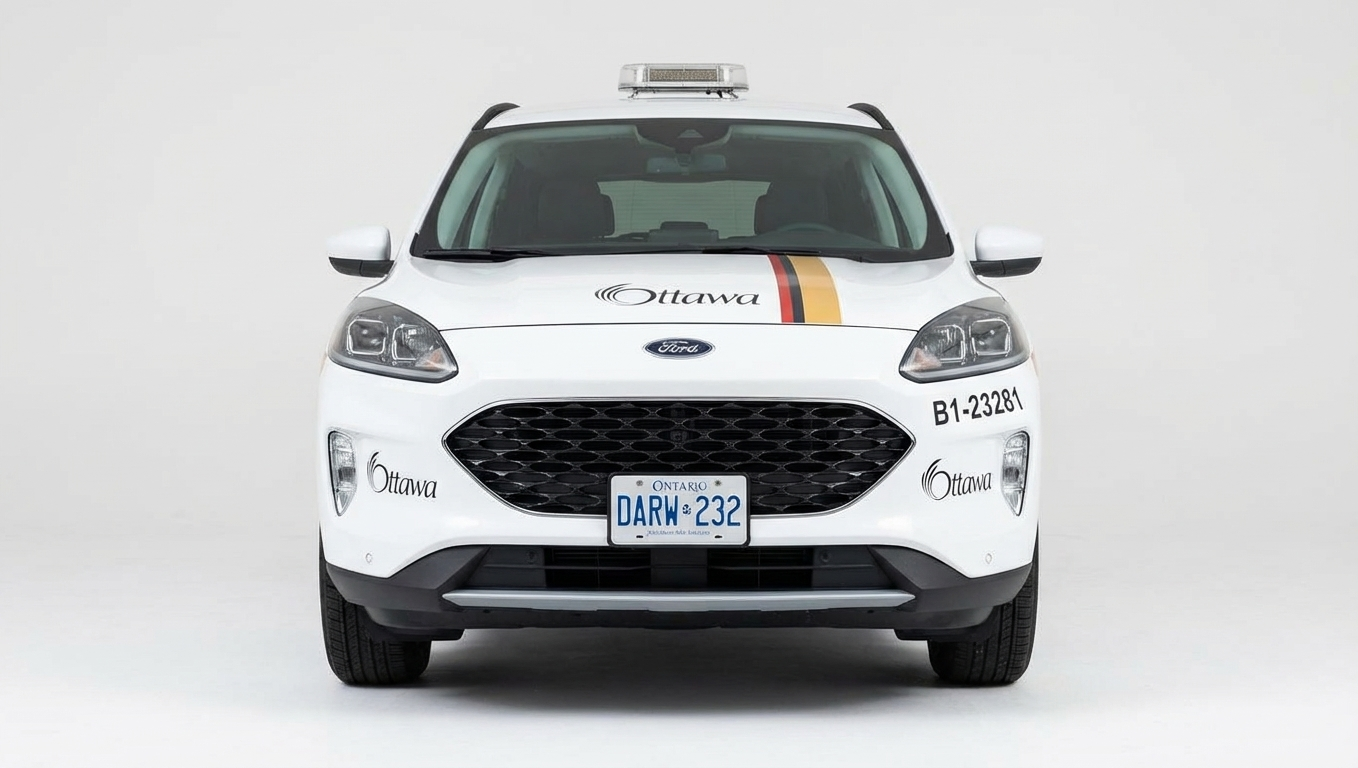
\includegraphics[width=\linewidth,height=0.40\textheight,keepaspectratio]{enforcement-reference-N.jpg}
		\column{0.25\textwidth}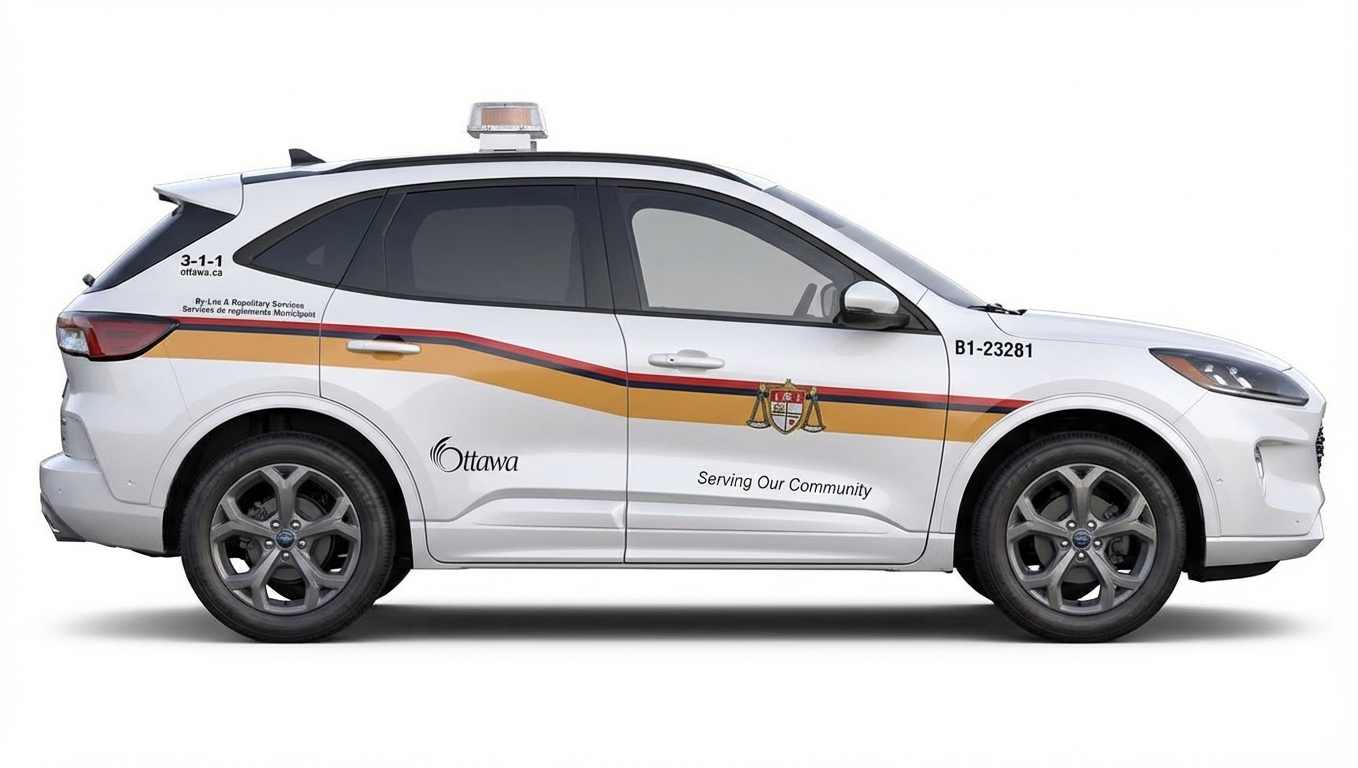
\includegraphics[width=\linewidth,height=0.40\textheight,keepaspectratio]{enforcement-reference-E.jpg}
		\column{0.25\textwidth}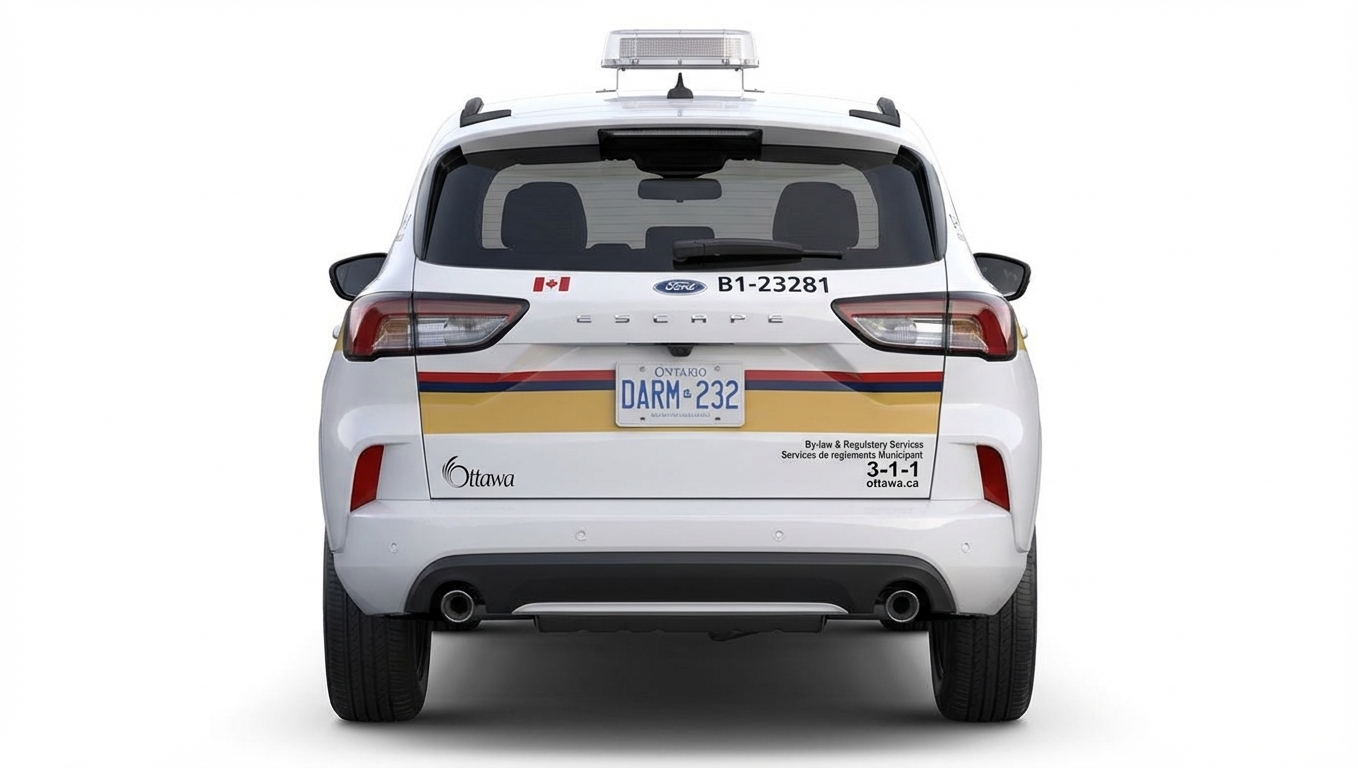
\includegraphics[width=\linewidth,height=0.40\textheight,keepaspectratio]{enforcement-reference-S.jpg}
		\column{0.25\textwidth}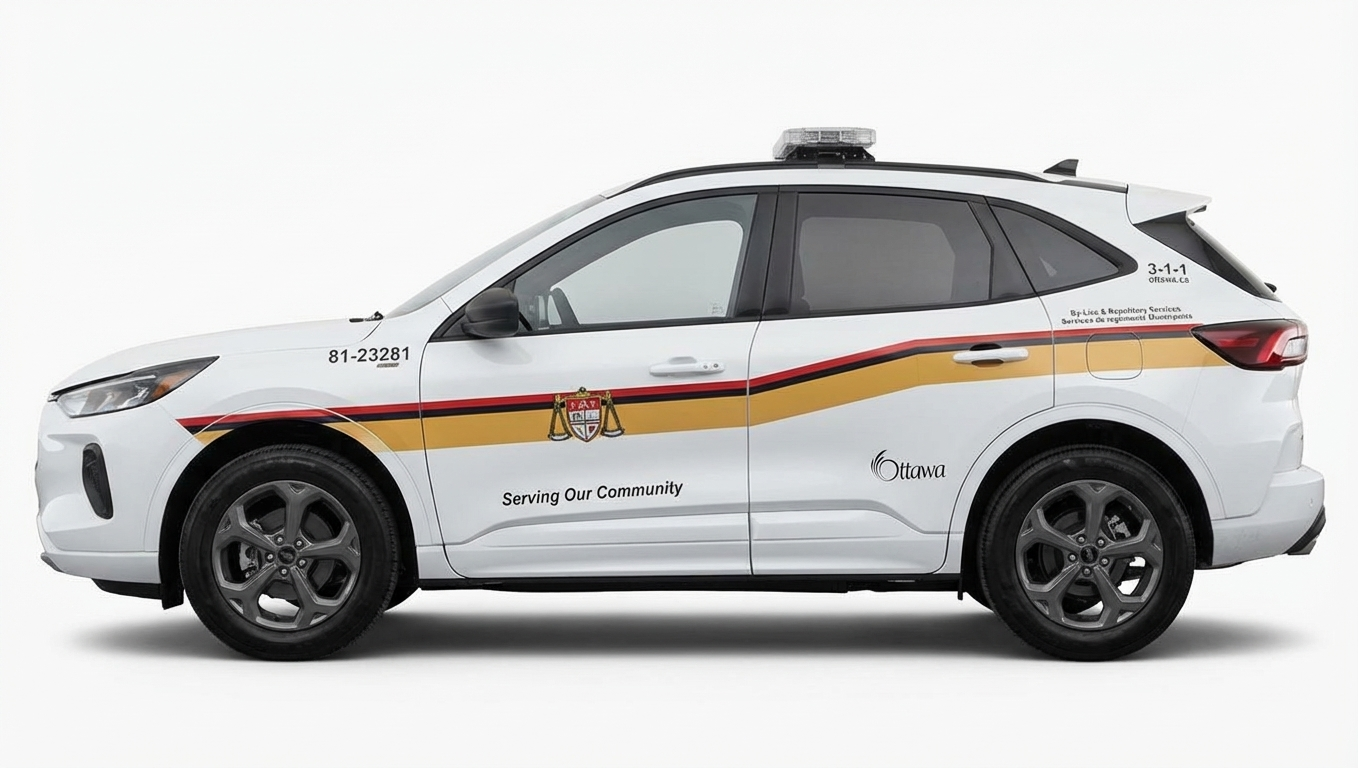
\includegraphics[width=\linewidth,height=0.40\textheight,keepaspectratio]{enforcement-reference-W.jpg}
	\end{columns}

	\vspace{0.18em}
	\begin{beamercolorbox}[wd=\linewidth,rounded=true,sep=0.7em,center]{block body}
		\textcolor{muted}{Four cardinal views of the same reference enforcement vehicle used for synth generation.}
	\end{beamercolorbox}
\end{frame}

\begin{frame}{Synthetic examples}
	\begin{columns}[T,onlytextwidth]
		\column{0.25\textwidth}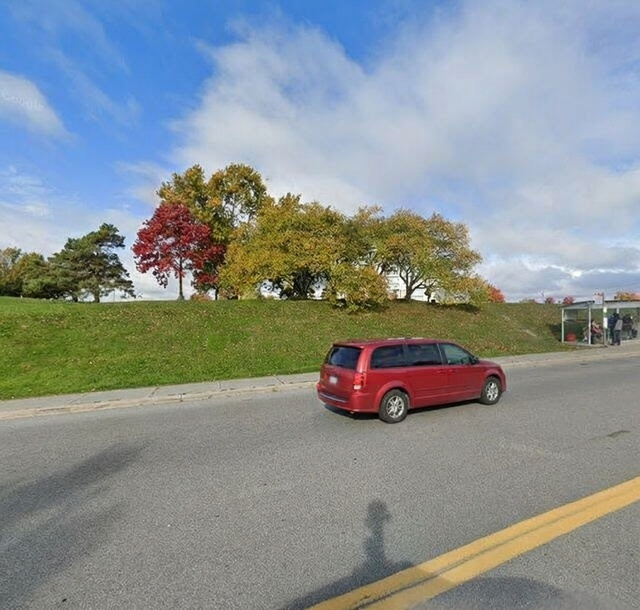
\includegraphics[width=\linewidth,height=0.40\textheight,keepaspectratio]{synthetic-random-vehicle.jpg}
		\column{0.25\textwidth}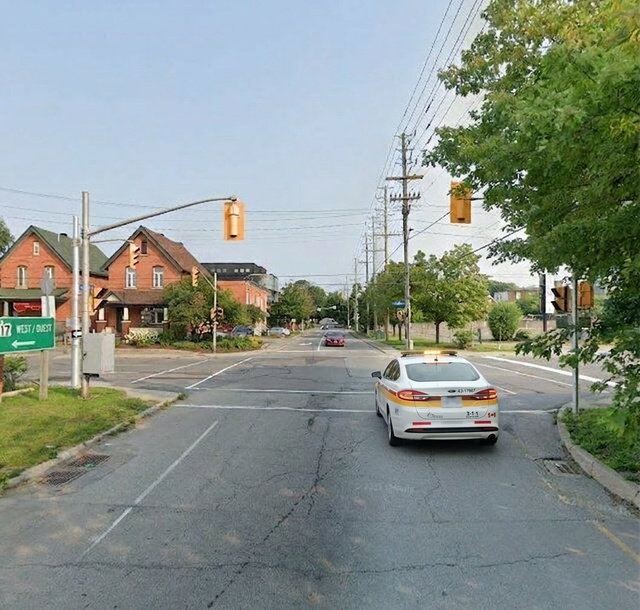
\includegraphics[width=\linewidth,height=0.40\textheight,keepaspectratio]{synthetic-enforcement.jpg}
		\column{0.25\textwidth}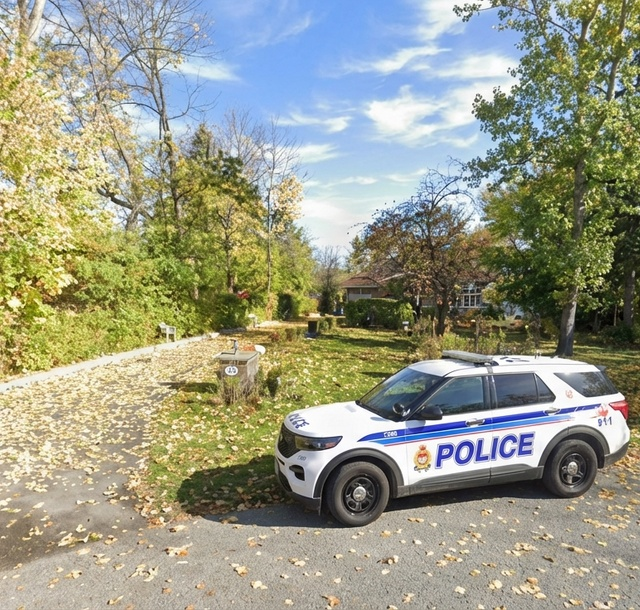
\includegraphics[width=\linewidth,height=0.40\textheight,keepaspectratio]{synthetic-police-old.jpg}
		\column{0.25\textwidth}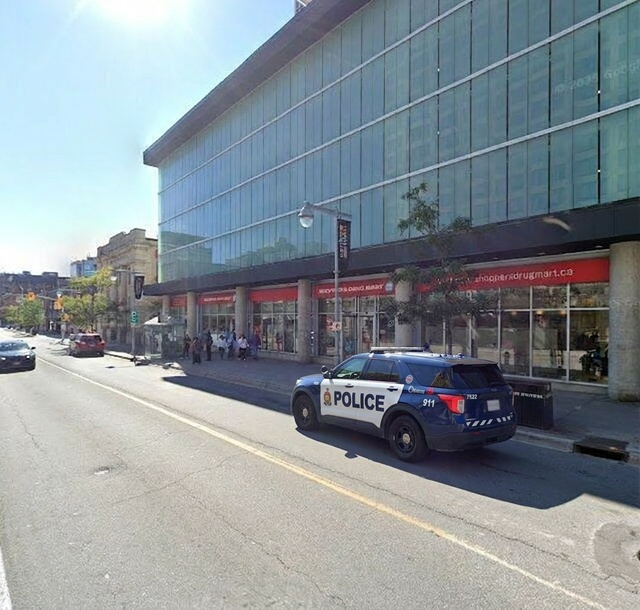
\includegraphics[width=\linewidth,height=0.40\textheight,keepaspectratio]{synthetic-police-new.jpg}
	\end{columns}

	\vspace{0.18em}
	\begin{beamercolorbox}[wd=\linewidth,rounded=true,sep=0.7em,center]{block body}
		\textcolor{muted}{Four variants, one goal: believable road context and clean vehicle placement.}
	\end{beamercolorbox}
\end{frame}

\begin{frame}{Assisted labelling}
	\centering
	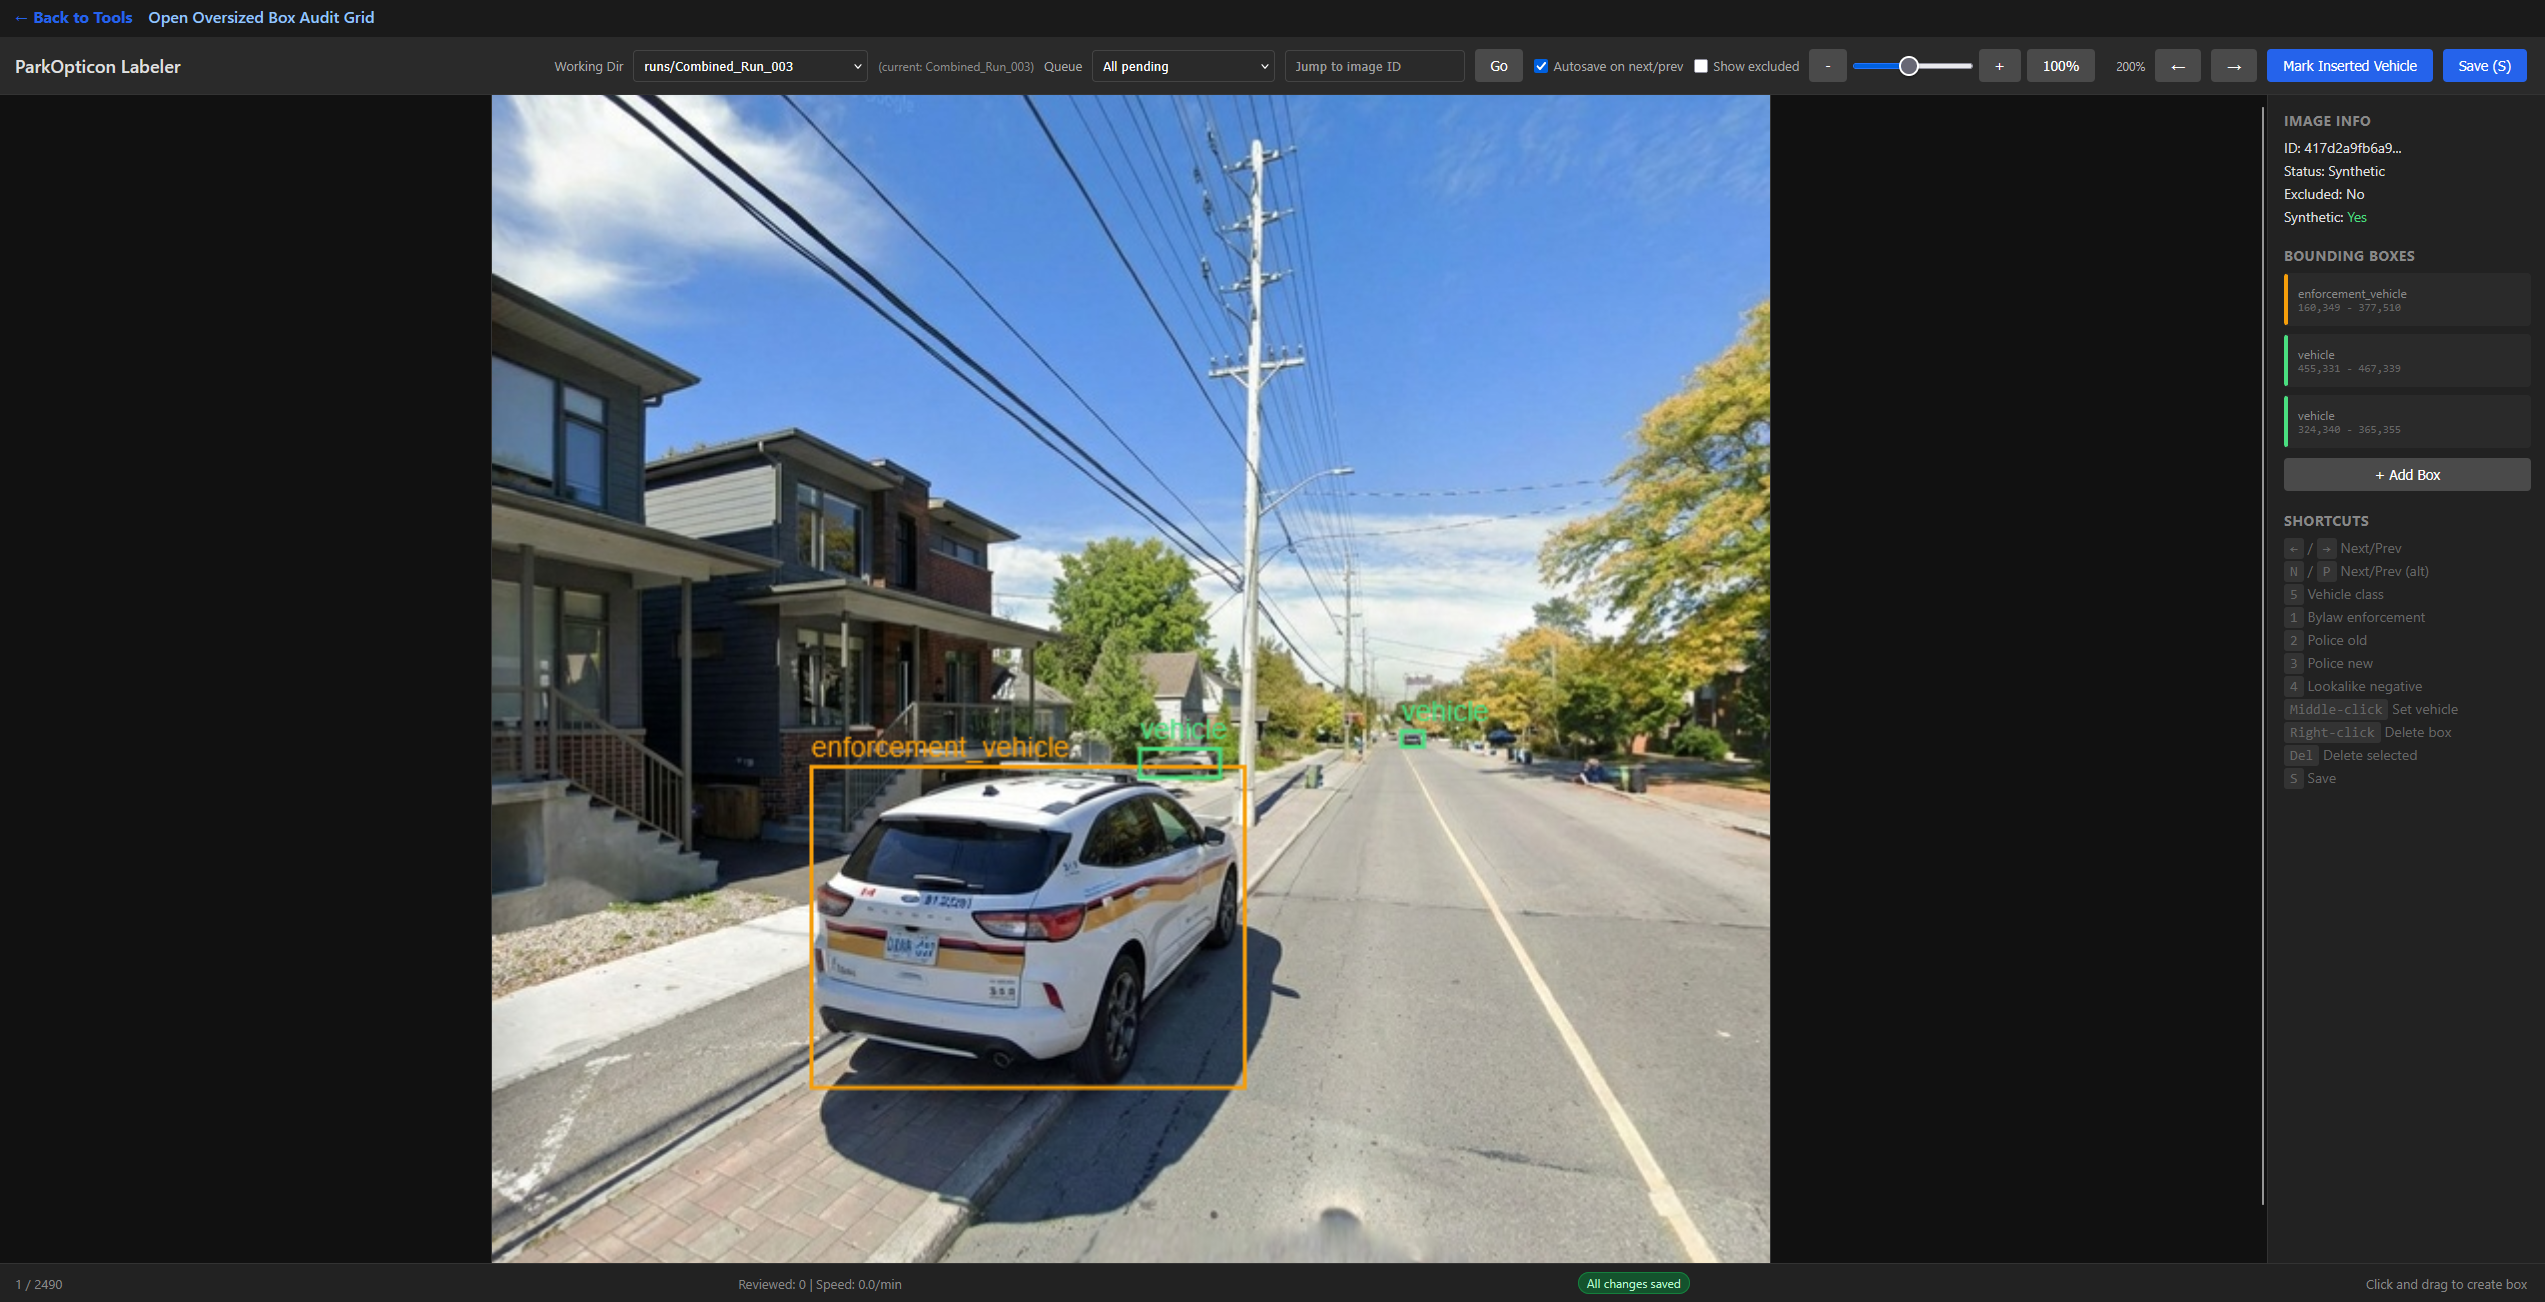
\includegraphics[width=1.03\linewidth,height=0.37\textheight,keepaspectratio]{labeller-ui.png}

	\vspace{0.52em}
	\begin{columns}[T,onlytextwidth]
		\column{0.36\textwidth}
		\begin{beamercolorbox}[wd=\linewidth,rounded=true,sep=0.72em,center]{block body}
			\textcolor{muted}{\scriptsize Reviewed}\par\vspace{0.30em}
			{\Large\bfseries 2,726 files}\par\vspace{0.42em}
			\textcolor{muted}{\scriptsize Human-final}\par\vspace{0.30em}
			{\Large\bfseries 19.8\% of items}
		\end{beamercolorbox}

		\column{0.58\textwidth}
		\begin{block}{How it worked}
			\begin{itemize}
				\item Prelabeller handled the first pass.
				\item Gating removed easy negatives.
				\item Humans only checked the tricky cases; light review took ~3s/file.
			\end{itemize}
		\end{block}
	\end{columns}

	\vspace{0.10em}
	\begin{beamercolorbox}[wd=\linewidth,rounded=true,sep=0.55em,center]{block body}
		{\small\bfseries Assisted labelling turned a full manual pass into fast targeted QA.}
	\end{beamercolorbox}
\end{frame}

\begin{frame}{Class folding insight}
	\begin{columns}[T,onlytextwidth]
		\column{0.37\textwidth}
		\begin{block}{Before}
			\begin{itemize}
				\item \texttt{lookalike\_negative} blurred the boundary.
				\item Similar vehicles split the signal.
			\end{itemize}
		\end{block}

		\vspace{0.25em}
		\begin{block}{After folding into \texttt{vehicle}}
			\begin{itemize}
				\item Labels got simpler.
				\item The detector got cleaner.
				\item Metrics improved sharply.
			\end{itemize}
		\end{block}

		\column{0.57\textwidth}
		\vspace{0.15em}
		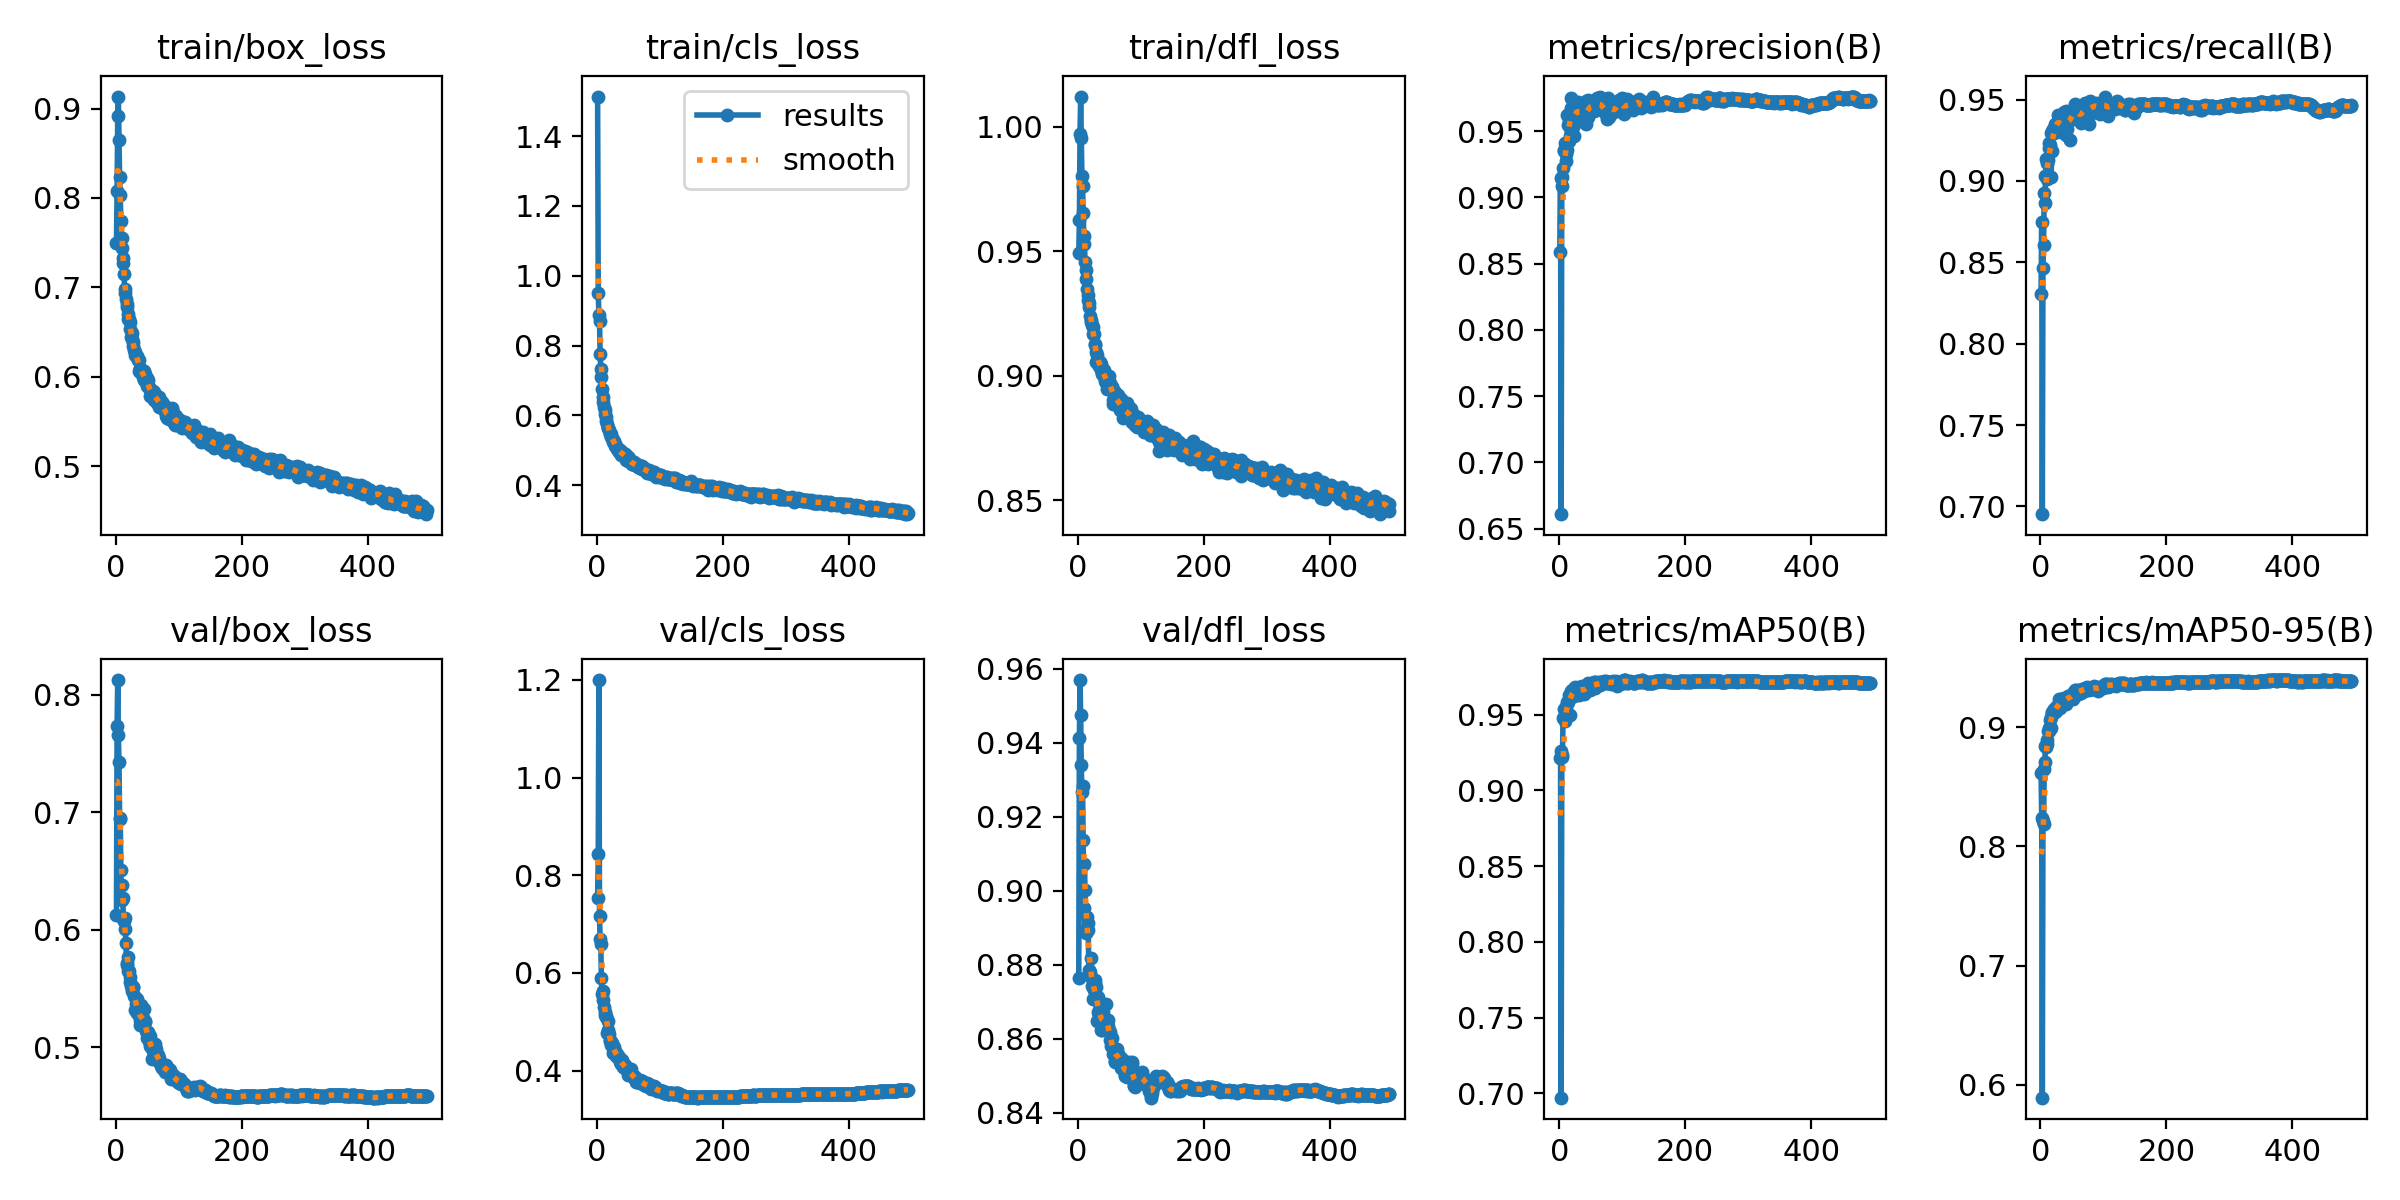
\includegraphics[width=\linewidth,height=0.54\textheight,keepaspectratio]{run_20260406/results.png}
	\end{columns}
\end{frame}

\begin{frame}{Results}
	\begin{columns}[T,onlytextwidth]
		\column{0.48\textwidth}
		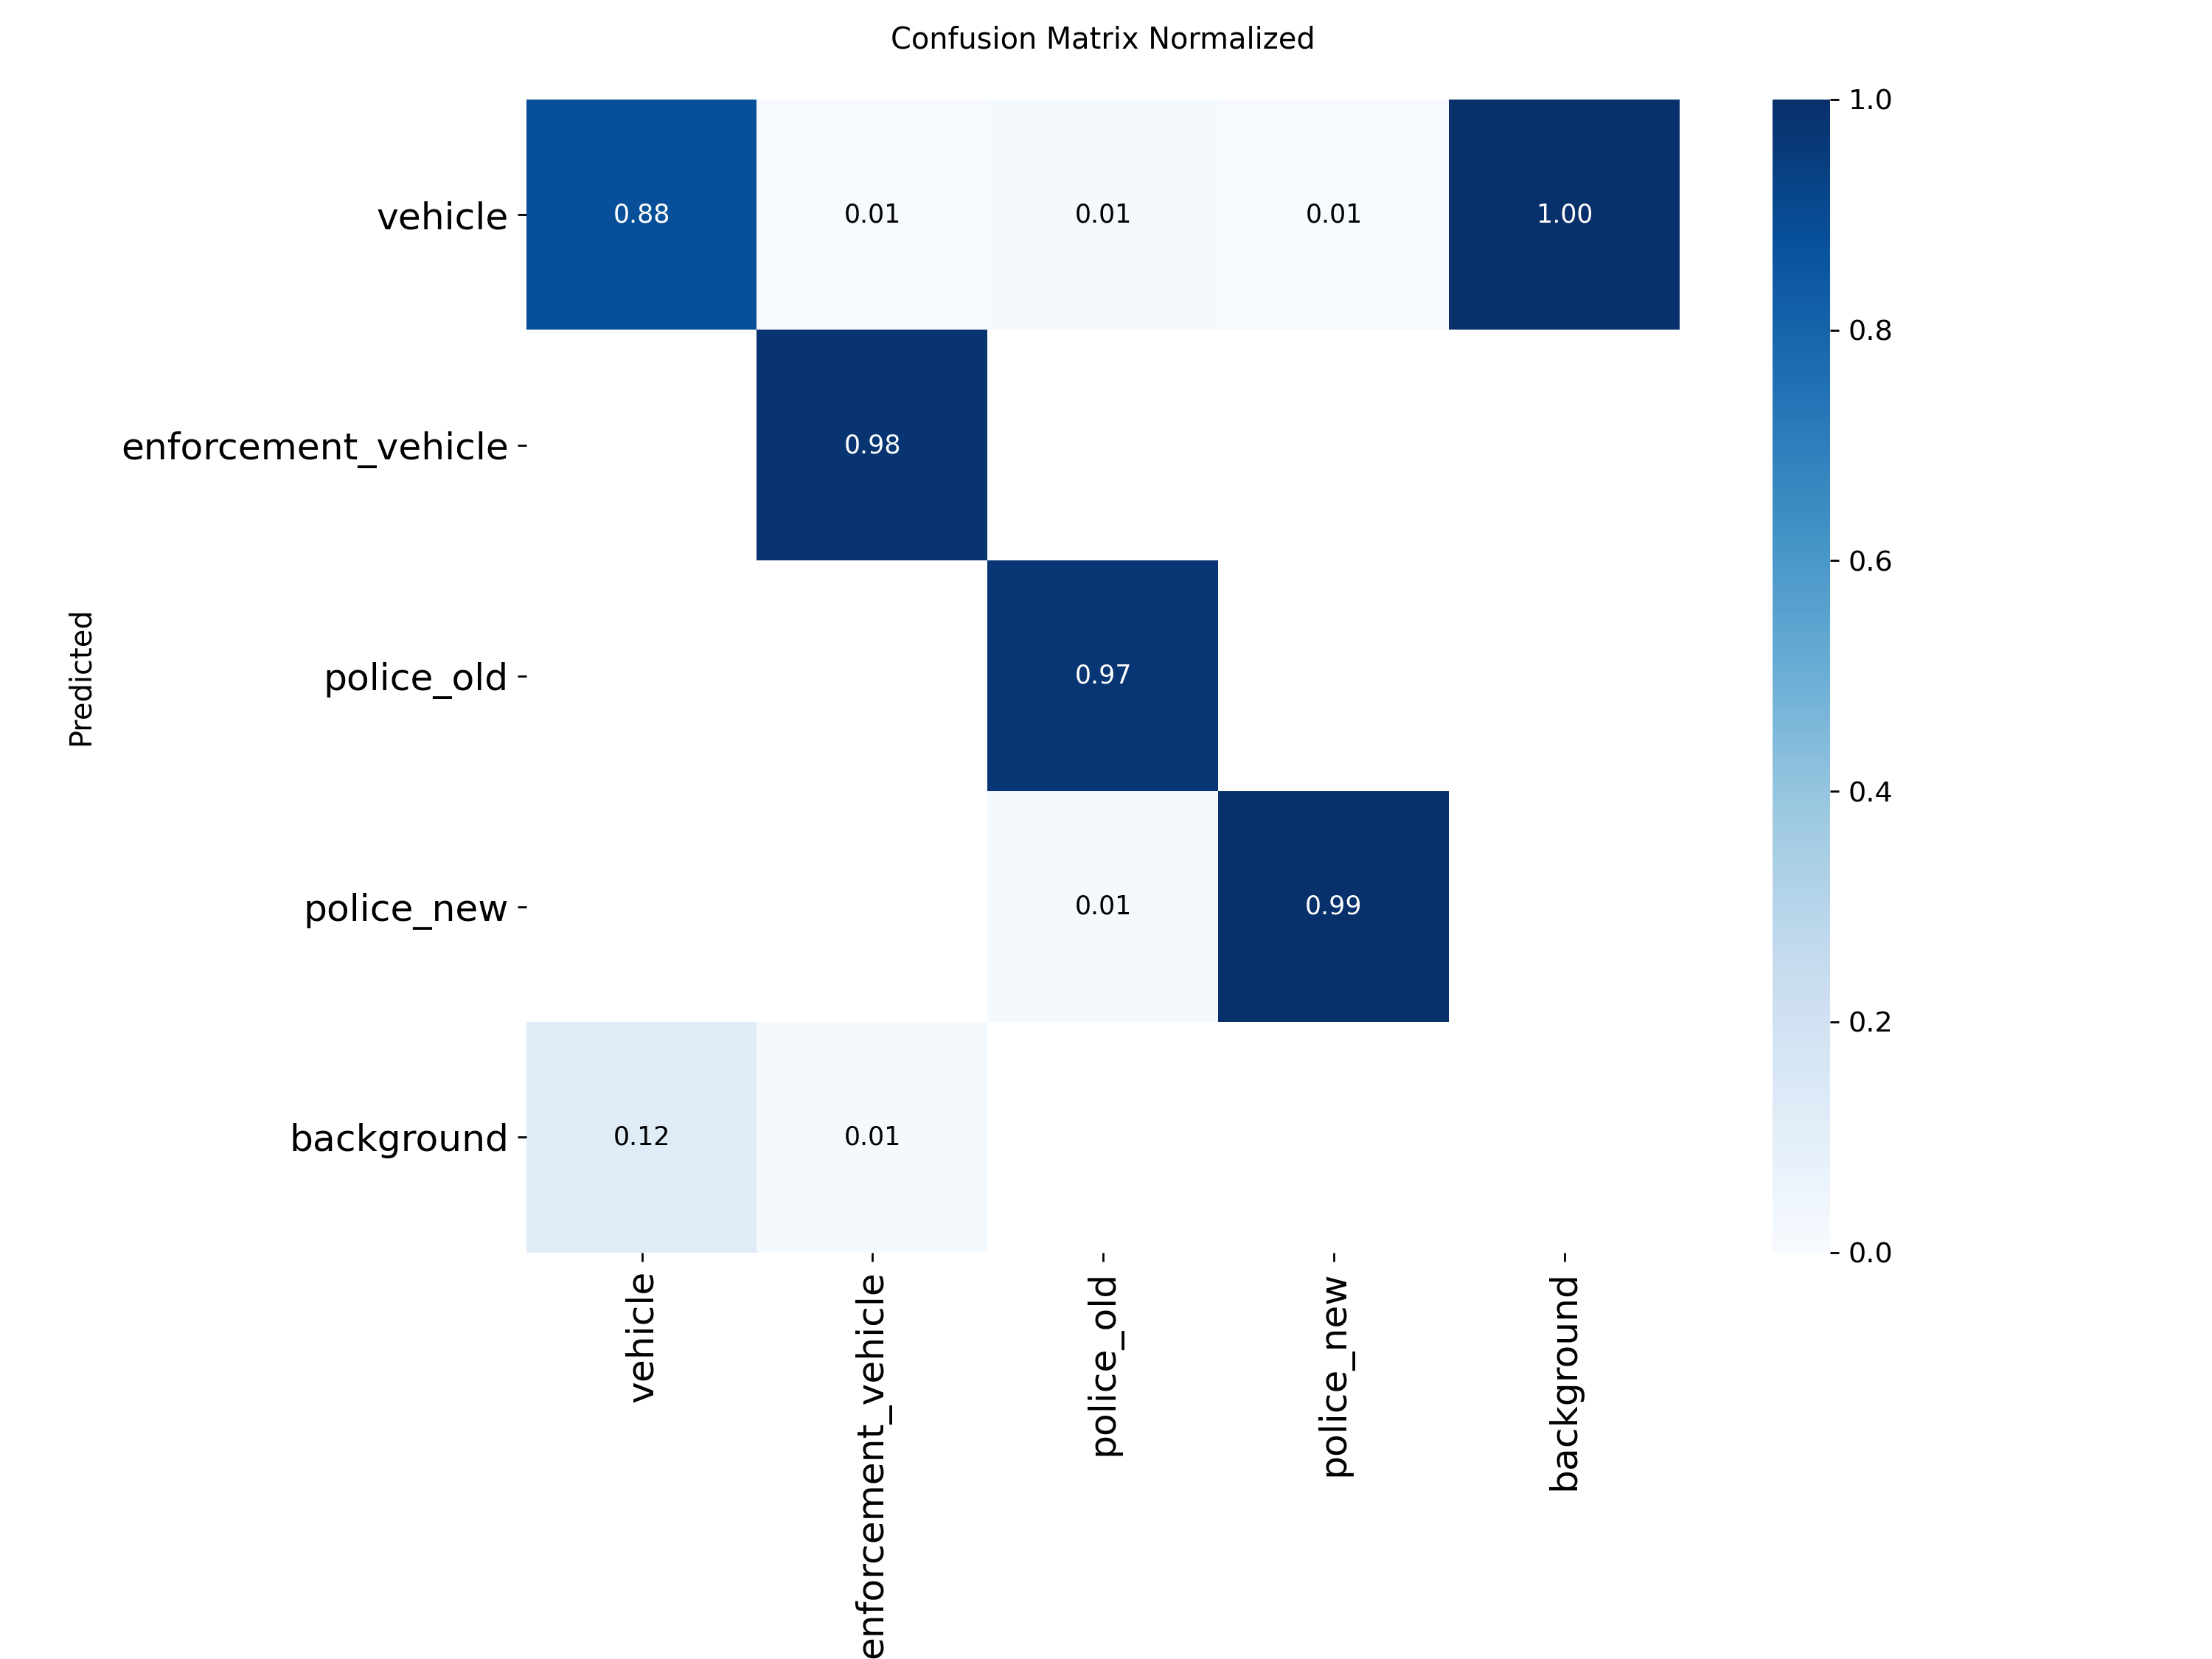
\includegraphics[width=\linewidth,height=0.44\textheight,keepaspectratio]{run_20260406/confusion_matrix_normalized.png}

		\column{0.48\textwidth}
		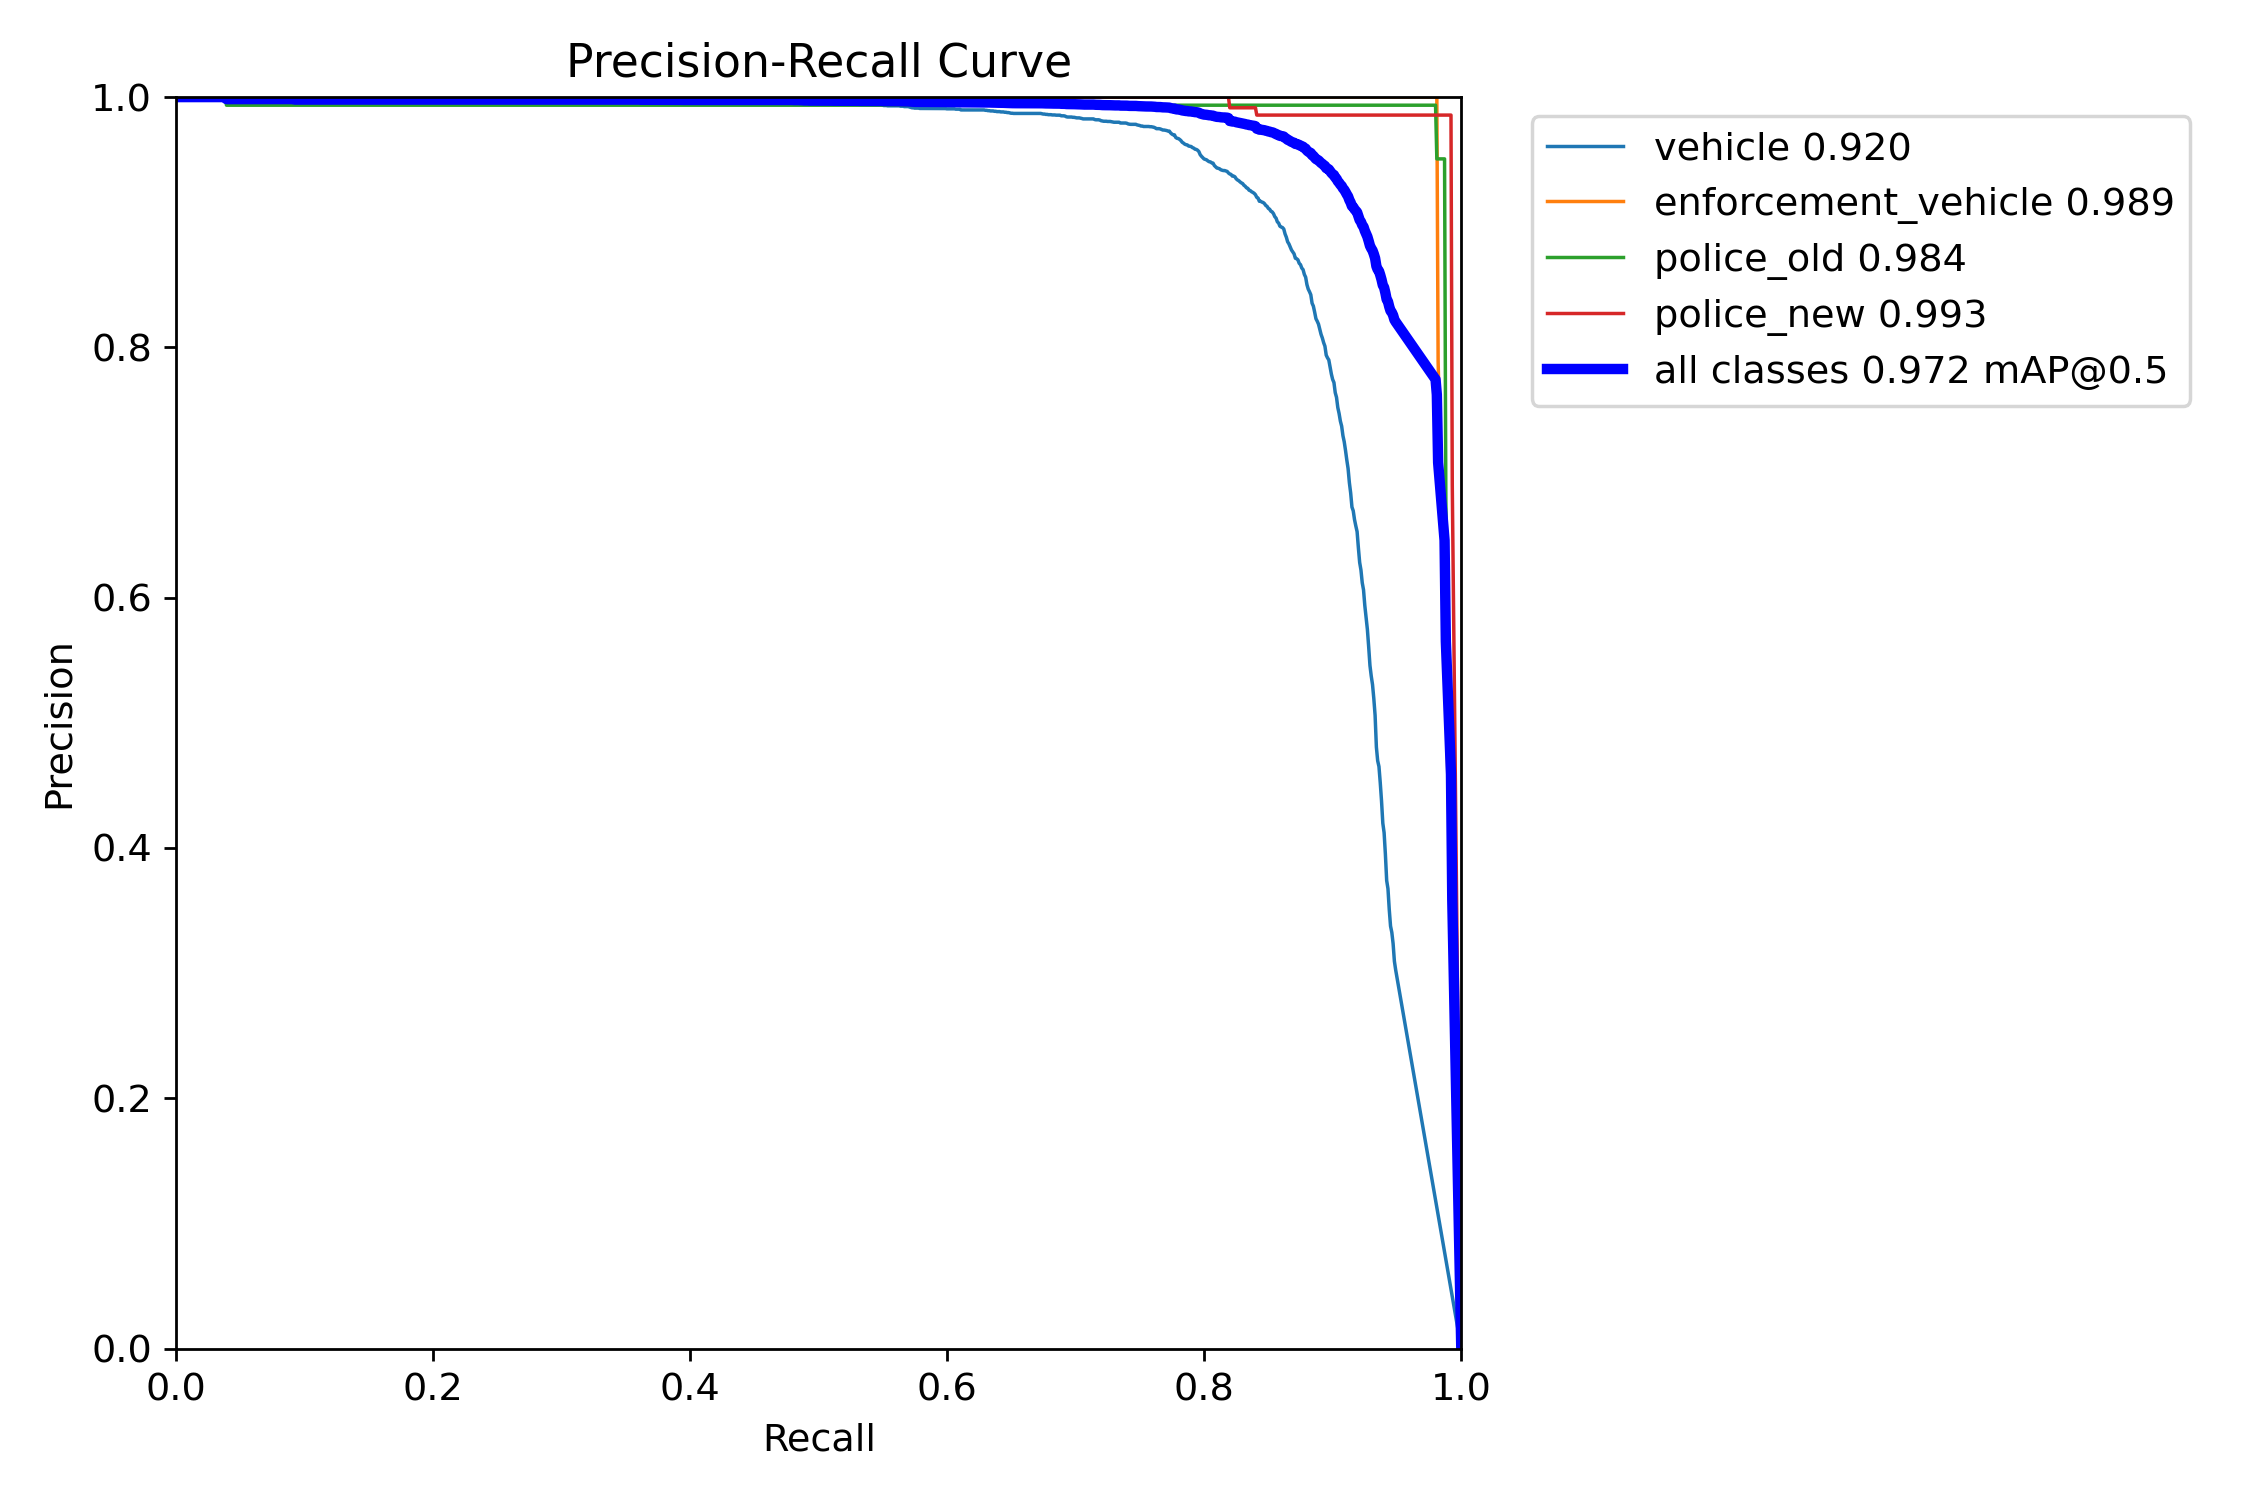
\includegraphics[width=\linewidth,height=0.44\textheight,keepaspectratio]{run_20260406/BoxPR_curve.png}
	\end{columns}

	\vspace{0.20em}
	\begin{beamercolorbox}[wd=\linewidth,rounded=true,sep=0.65em,center]{block body}
		{\small\bfseries P 0.976 \quad | \quad R 0.946 \quad | \quad mAP50 0.973 \quad | \quad mAP50--95 0.939}
	\end{beamercolorbox}
\end{frame}

\begin{frame}{Scale}
	\begin{columns}[T,onlytextwidth]
		\column{0.25\textwidth}\bigmetric{Final images}{9,987}{all processed data}
		\column{0.25\textwidth}\bigmetric{Panorama groups}{1,060}{split safely by group}
		\column{0.25\textwidth}\bigmetric{Reviewed files}{2,726}{selective human QA}
		\column{0.25\textwidth}\bigmetric{Review time}{2h16m}{at 3s/file}
	\end{columns}

	\vspace{0.55em}
	\begin{beamercolorbox}[wd=\linewidth,rounded=true,sep=0.75em]{block body}
		\textcolor{muted}{Run isolation and group-aware splitting kept siblings together and reduced leakage risk.}
	\end{beamercolorbox}
\end{frame}

\begin{frame}{Gemini cost}
	\begin{alertblock}{Actual spend}
		\centering
		{\Huge\bfseries \$2,497}\par
		\vspace{0.2em}
		{\large Planned: \$500--\$600}\par
	\end{alertblock}

	\vspace{0.45em}
	\begin{beamercolorbox}[wd=\linewidth,rounded=true,sep=0.8em]{block body}
		\textcolor{muted}{\small Planned estimate}\par
		{\Large\bfseries \$500--\$600}\par
		\vspace{0.15em}
		\textcolor{muted}{\small Manual equivalent: \$15,000--\$30,000 for image collection, compositing, and annotation}\par
		\vspace{0.10em}
		\textcolor{muted}{\small One-line takeaway: image collection would dominate the manual budget.}
	\end{beamercolorbox}
\end{frame}

\begin{frame}{Lessons and next steps}
	\begin{block}{Lessons}
		\begin{itemize}
			\item Synthetic-only training can work well.
			\item Run isolation and split discipline mattered.
			\item Selective review beat exhaustive annotation.
		\end{itemize}
	\end{block}

	\vspace{0.2em}
	\begin{alertblock}{Next step}
		Train an ESPdet model for ESP-32 deployment next --- basically plug-and-play for the next phase.
	\end{alertblock}

	\vspace{0.25em}
	\begin{center}
		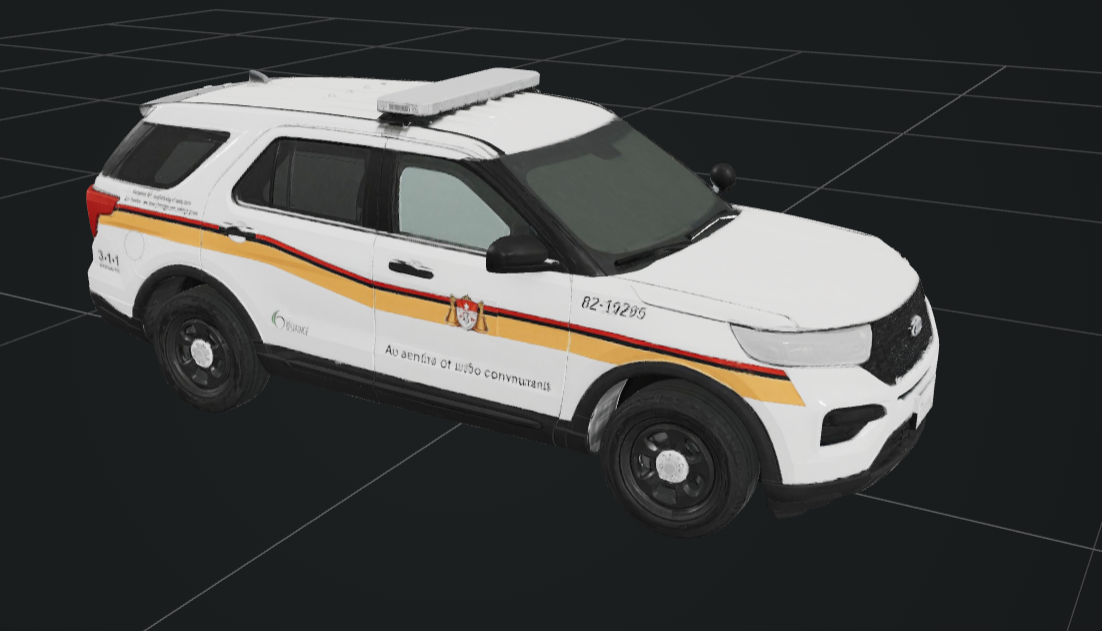
\includegraphics[width=0.56\linewidth,height=0.24\textheight,keepaspectratio]{3d-model.png}
	\end{center}
\end{frame}

\end{document}
